\section{Process Design}
This section features pseudocode for the vast array of processes that will be used throughout the system. Due to the functional paradigm with which the application will be programmed, many of these processes (referred to hereafter as functions) will be used multiple times, and combined with other functions. To aid in readability, pseudocode for each function will be listed only once. The following is a list of all the processes that will be used:

\begin{itemize}
\item Create, read, update and delete quizzes.
\item Display time until the quiz begins.
\item Calculate suitable colour pallete for each house.
\item Calculate the number of house points for each packet.
\item Calculate the most common answer in each house / year.
\item Keep state of quiz in sync between each device.
\end{itemize}

\subsection{API Test Runs}
These are the tests for the restful API. The API acts as a means of communicating with the database. In order to do so, certain requests - either GET, POST, PUT or DELETE - are sent to an address; in this case, \textit{/api/quizzes}. The API then looks at the request type that was sent, along with any other data that came with it, and performs the appropriate operation, be that showing a list of all quizzes, showing a specific quiz, or updating a quiz.

\subsubsection{api.spec.js} % (fold)
\label{ssub:api_spec_js}
\lstinputlisting[language=javascript, caption=Unit tests for the API.]{../test/api.spec.js}
\begin{figure}[h!]
  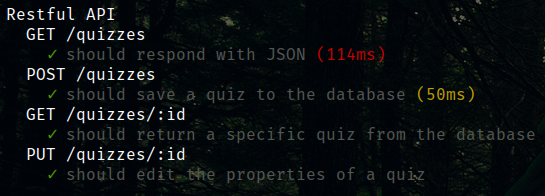
\includegraphics[scale=0.55]{testing/api/api}
  \caption{Test outcome for api.spec.js 1}
\end{figure}
% subsubsection api_spec_js (end)

As can be seen by the little green ticks, all the different HTTP methods passed, proving that the API is working correctly, and thereby allowing requests to be sent from throughout the application. \textit{Success.}


\subsection{Validation Test Plan} % (fold)
\label{sub:validation_testing}
This subsection displays the test data that will be used to test the validation used throughout the system, and the responses that should occur when the data is entered.

\subsubsection{Only Integers in Question and Break Fields} % (fold)
\label{ssub:only_numbers_in_question_and_break_fields}
This validation will ensure that the question and break fields only accept integers, as they are used in the scheduling of the quiz and so must be validated.
\begin{enumerate}
  \item Enter ``10'' into the question length and break fields. (\textit{Typical})\\\\
  \textit{Expected result}: Nothing should happen, as the data is as expected.\\

  \item Attempt to enter ``abc'' into the question length and break fields. (\textit{Extreme})\\\\
  \textit{Expected result}: The fields should prevent such characters being inserted.\\

  \item Do not enter anything into the fields and save. (\textit{Null})\\\\
  \textit{Expected result}: Nothing should change, as the previous values will not have been updated.\\
\end{enumerate}
% subsubsection only_numbers_in_question_and_break_fields (end)

\subsubsection{Minimum Question Length} % (fold)
\label{ssub:minimum_question_length}
Students should be given a minimum of five seconds to answer a question. This validation ensures that this value is enforced when setting a custom question length.
\begin{enumerate}
  \item Enter ``10'' into the question length field. (\textit{Typical})\\\\
  \textit{Expected result}: Nothing should happen, as the data is as expected.\\

  \item Enter ``3'' into the question length field. (\textit{Extreme})\\\\
  \textit{Expected result}: A message should appear, stating that questions must be at least 5 seconds.\\

  \item Enter ``-8238'' into the question length field. (\textit{Erroneous})\\\\
  \textit{Expected result}: A message should appear, stating that questions must be at least 5 seconds.
\end{enumerate}
% subsubsection minimum_question_length (end)

\subsubsection{Minimum Break Length} % (fold)
\label{ssub:minimum_question_length}
Students should be given a minimum of one minute in a break. This validation ensures that this value is enforced when setting a custom break length.
\begin{enumerate}
  \item Enter ``5'' into the break length field. (\textit{Typical})\\\\
  \textit{Expected result}: Nothing should happen, as the data is as expected.\\

  \item Enter ``0.5'' into the break length field. (\textit{Extreme})\\\\
  \textit{Expected result}: A message should appear, stating that breaks must be at least 1 minute.\\

  \item Enter ``-8238'' into the break length field. (\textit{Erroneous})\\\\
  \textit{Expected result}: A message should appear, stating that breaks must be at least 1 minute.
\end{enumerate}

\subsubsection{One Correct Answer Per Question} % (fold)
\label{ssub:one_correct_answer_}
Each question can only have one correct answer. This aspect of the validation will ensure that only one answer per question can be marked as correct in the quiz editor.

\begin{enumerate}
  \item Create a new quiz.
  \item Mark the first answer as correct by clicking on the tick icon.\\\\
  \textit{Expected result}: The tick in the first answer should now be highlighted, and the previous tick should be pale.
\end{enumerate}
% subsubsection one_correct_answer_ (end)
% subsection validation_testing (end)

\subsubsection{housePoints.js} % (fold)
\lstinputlisting[language=javascript, caption=Returns the number of house points earned from an answer.]{../src/libs/housePoints.js}
% subsubsection mostcommon_js (end)

